\chapter{Annotation Protocol, Datasets, and Software Solutions}
\label{datasets}

\resetfigpath{datasets}

In this chapter, we start by specifying the annotation protocol and emphasize its efficiency by comparing to the more traditional approaches.
We further enumerate the conditions of applicability that our annotation/segmentation frameworks will have to respect, and suggest a serie of medical sequences that will constitute our benchmarks.
In the last section, we present two software solutions that have been designed and implemented in the frame of this thesis.
The first is a flexible annotation software.
The second is a web platform that allows users to upload their annotations and images, so as to receive, after the computations are done, the segmentation results.

\textbf{Author contributions} The software solutions presented in this chapter combine the contributions of Severin Tobler, Jan Grossrieder, Philipp Gerber, Olen Andoni, and myself.
Severin Tobler, as part of his civil service, contributed to the coding of the annotation software, in particular, the design of the \gls{gui}, coding the video/volume decoding layers, and the documentation.
Jan Grossrieder, Philipp Gerber, and Olen Andoni all contributed equally to the coding of the web platform.

\textbf{My personal contributions include}:
\begin{itemize}
    \item Supervision and testing of both projects
    \item Coding parts of the annotation software: Decoding of videos and gaze-tracker integration
    \item Packaging of the annotation software for Linux platforms
    \item Coding parts of the web-platform: Frontend, backend, packaging
    \item Documentation of the web-platform
\end{itemize}

\section{Proposed annotation protocol and requirements}

In the present thesis, we devise solutions that allow to annotate medical sequences in a fast and intuitive manner, in an attempt to alleviate the bottleneck of scarcity of example data.

The proposed annotation protocol is the following.
The annotator is presented a video or volumetric sequence that plays on a screen, i.e. the frames unfold in an automatic manner.
As the sequence unfolds, the annotator is asked to point at the object of interest using a pointing device, such as a mouse, a tablet pen, or an eye-gaze tracker.
In contrast with the traditional approach, where the object must be manually segmented on each frame individually, the proposed protocol drastically reduces the annotation time.
In essence, our contribution ambitions an annotation time equal to the duration of the video/volume playback.
For example, assuming the sequence contains $100$ frames playing at $5fps$, the total annotation time is $20$ seconds.
In comparison, the traditional pixel-wise annotation task of a sequence of similar size could take anywhere from $10$ min. to $1$ hour, depending on the image modality and nature of object.

Concretely, we set the following requirements on the annotation protocol:
\begin{itemize}
  \item The annotator does not need to manually change the frame being annotated, e.g. by hitting a forward or backward key. The sequence automatically unfolds according to a pre-specified frame-rate.
  \item The annotator handles a single pointing device, which he/she uses to indicate the location of the object of interest.
  \item The annotator must be to annotate the sequence in a single go, i.e. he/she does not need to review annotations and modify them manually afterwards.
\end{itemize}

The segmentation method must be functional in a variety of situations, namely produce acceptable accuracy for:
\begin{itemize}
  \item Both videos and volumetric sequences.
  \item Both color and grayscale images.
  \item Various kind of image modality, e.g. \gls{mri} and \gls{ct}.
  \item Various levels of noise, perturbations, and lightning artifacts.
  \item Various nature of object, i.e. size, shape, appearance.
  \item The object can be made of several parts that are not contiguous, i.e. an \gls{mri} brain scan with several tumors.
\end{itemize}


\section{Datasets}

We now introduce the datasets that have been used during the elaboration and testing of the proposed solutions.
Note that as the range of possibilities is huge, we choose to restrict ourselves to $4$ types of sequences.
These, however, cover the entirety of the proposed spectrum of requirements.

We now describe them in detail and give each type a short name that will be used in the remaining of this thesis:

\begin{itemize}
  \item \textbf{Tweezer}: Surgical instruments during an endoscopic procedure, where the instrument is object of interest.
    The background is relatively homogeneous, while the instrument moves accross the frame both in translation and rotation.
    The sequences are taken from the MICCAI EndoVision Challenge \cite{EndoChall}.
    Each sequence is around $120$ frames long, i.e. represent $\sim 5s$ of video acquired at $25$ fps.
  \item \textbf{Cochlea}: Volumetric \Gls{ct} scans of the inner-ear where the cochlear labyrinth is to be segmented. These are acquired according to different protocols, and therefore show important variations in gray-scale level, orientation, as well as sizes. Furthermore, the object of interest is composed of different parts that split and merge, thereby making this type the most challenging.
    Each scan contains $\sim 100$ slices.
  \item \textbf{Slitlamp}: Microscopic video of the retina where the optic nerve is to be segmented. The videos have been acquired using a slitlamp instrument.
    The optic nerve is of rather small size. The background often shows important artifacts, in the form of yellow and blue beams, which sometime overlap with the object of interest. The movement of the optic nerve is often very jerky.
    Each video contains $\sim 120$ frames acquired at $25$ fps.
  \item \textbf{Brain}: Transverse \gls{mri} scans of brains where the tumor is object of interest. The sequences are taken randomly from the Brain Tumor Segmentation Challenge (BRATS) public database \cite{BRATSChall}.
    Scans are acquired using the same \gls{mri} protocol, but with different scanners, thereby showing wide variety of contrast and color.
    The tumors have varying size, colors, and shapes. Sometimes, the same scan shows several tumors on the same slice.
    Each scan contains $\sim 80$ frames.
\end{itemize}

In Fig. \ref{fig:dset_previews}, we show example frames for each type.

\begin{figure}
\centering
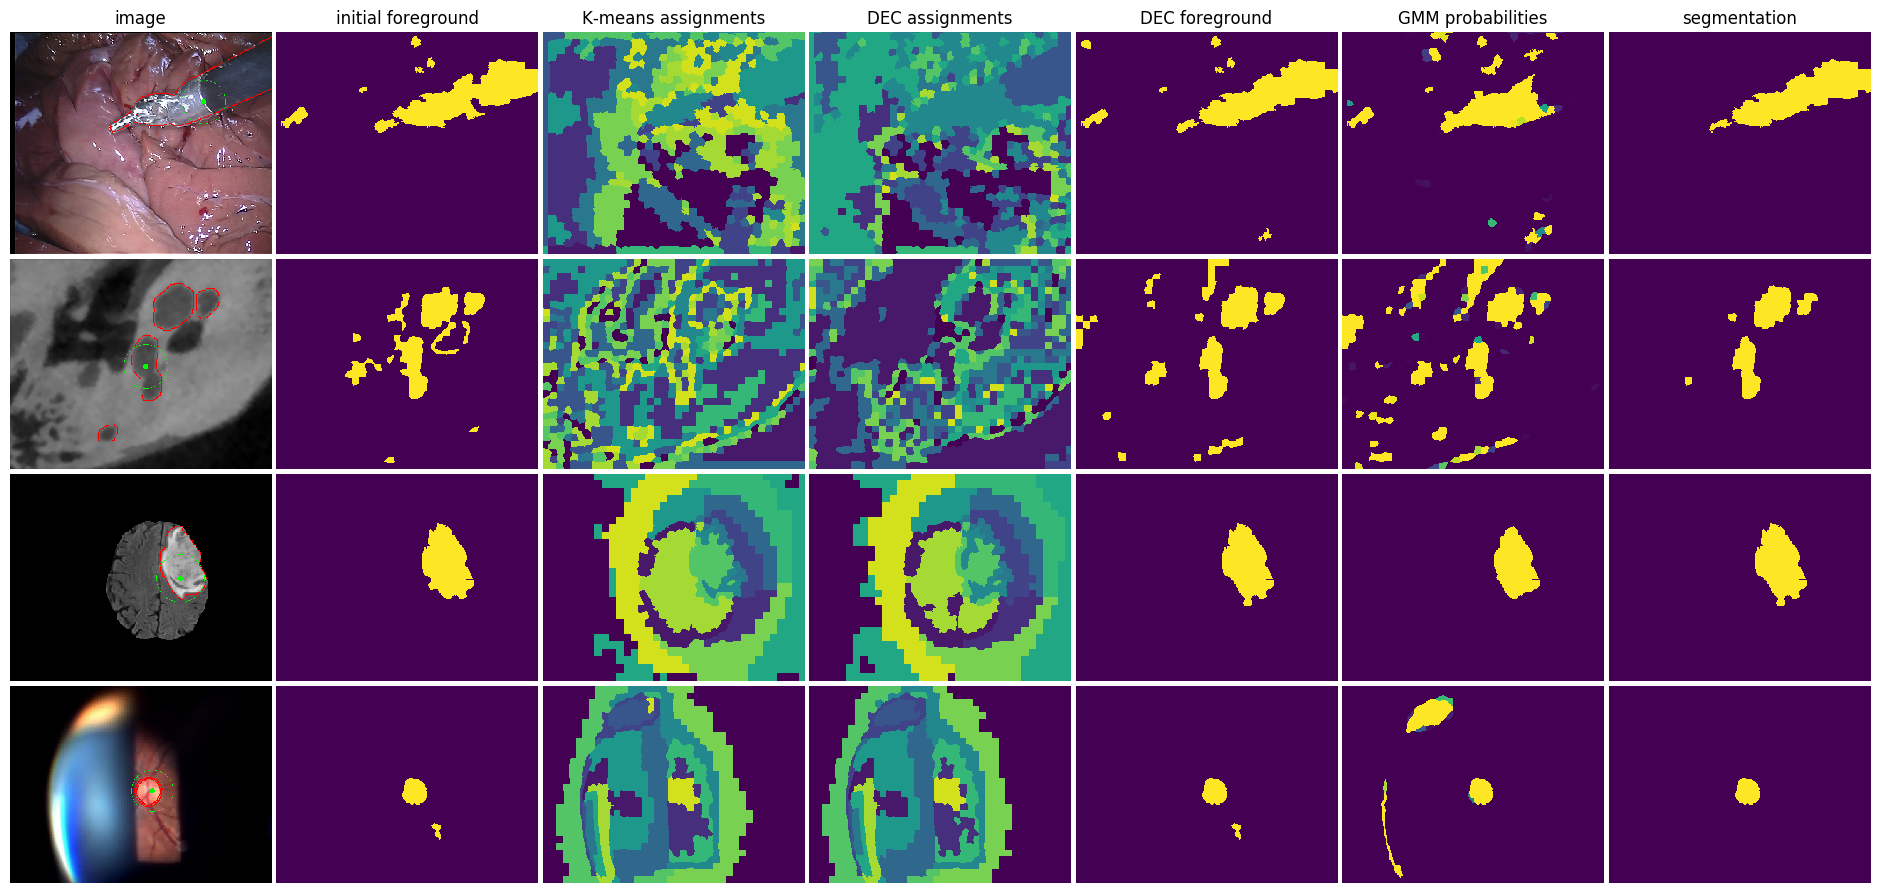
\includegraphics[width=0.99\textwidth]{prevs.png}
\caption{Example of objects of interest in different video and volumetric modalities. Each type contains 4 sequences. We show a single frame per sequence.
  From top to bottom: Tweezer, Cochlea, Slitlamp, and Brain}
\label{fig:dset_previews}
\end{figure}


\section{Annotation Software and Web Platform}
In the frame of this thesis, a flexible and elegant annotation software was developed that supports as pointing device a traditional mouse, a pen compatible with touch-screens, as well as a backend interface that allows to connect a eye-gaze tracker through the USB port.
Our second contribution is a web platform.
Its goal is to allow a user to upload a sequence (video or volumetric), along with his/her annotations, as generated with the annotation software.
A backend module then triggers an instance on a cluster (potentially equipped with a \gls{gpu}) that will produce the segmentation.
Once the latter step is complete, the user is able to download the generated pixel-wise segmentation.
We now describe both contributions.

\subsection{Annotation Tool}
\label{sec:anna}

We design an annotation software that supports the following features.

\begin{itemize}
    \item We want the software to be cross-platform, i.e. run on the most popular operating systems, i.e. Windows, MacOS, and Linux.
    \item We wish to have a polished and user-friendly \gls{gui}.
    \item The software must support the most standard types of files, i.e. popular video formats and DICOM.
    \item We further wished to experiment on using an eye-gaze tracker in place of standard pointing devices.
\end{itemize}

To guarantee cross-platform compatibility, we choose the Qt5 framework \cite{eng16}, which relies on C++ and provides convenient widgets out of the box, such as drop-down menus, a file dialog, and sliders.

So as to decode and display both standard videos and DICOMs, we resort to two solutions.
To support standard video compression formats, we resort to the OpenCV library \cite{opencv}.
For DICOM, the de-facto standard in medical imaging hardware, our software leverages the ITK library \cite{johnson15}.

Regarding the acquisition of user's annotation, the mouse and tablet-pen inputs are naturally handled by the Qt framework.
For acquisition using the eye-gaze tracker, we implement a module that is compatible with the proprietary backend given by the manufacturer of the tracker \cite{eyetribe}.

The typical annotation workflow is the following:

\begin{itemize}
  \item[-]{Provide as input a volume/video, either from file drop-down menu are by drag-and-drop.}
  \item[-]{Optional: Set the framerate at which the sequence will play (right knob on Fig. \ref{fig:anna}).}
  \item[-]{Optional: Connect the software to the eye-gaze tracker server. The tracker will then act as a secondary mouse.}
  \item[-]{Hit the play button (or space-bar if available). The sequence unfolds.}
  \item[-]{Annotate:}
    \begin{itemize}
      \item[-]{When using mouse: Simply click on the desired region.}
      \item[-]{When using gaze-tracker: Place gaze on region and use right button (Fig. \ref{fig:anna}) to activate the recording of locations.}
    \end{itemize}
  \item[-]{When annotation is done, save them in \gls{csv} format.}
\end{itemize}

\begin{figure}[!htpb]
  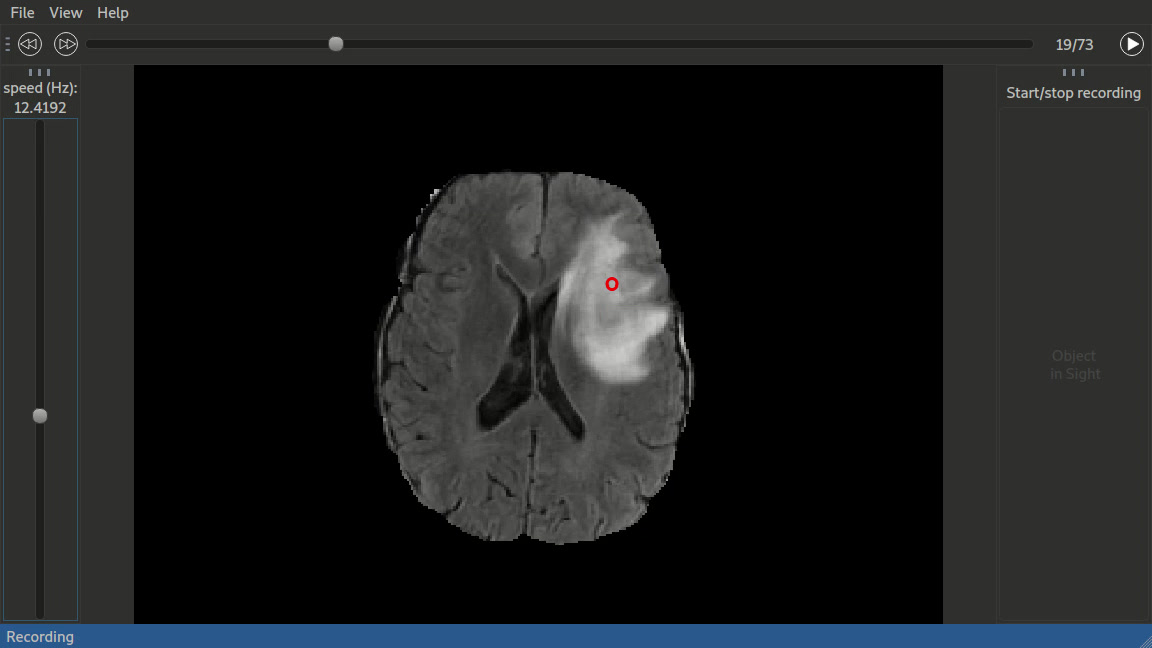
\includegraphics[width=0.99\textwidth]{anna0.png}
  \caption{Example screenshot of our annotation tool showing a Brain sequence.
  The current annotation point is shown in red.}
  \label{fig:anna}
\end{figure}

We make our source code publicly available at \url{https://github.com/aimi-lab/Anna}.
In Fig. \ref{fig:anna}, we show an example screenshot.


\subsection{Web platform}
The segmentation methods presented in the next chapters sometimes require important computational resources, namely a \gls{gpu} for the training of deep networks.
We therefore provide a way for users to upload their data along with the corresponding 2D locations to a server that will perform the necessary computations remotely and send back segmentation results when they are available.
Concretely, we develop a web interface that provides:

\begin{itemize}
  \item[-]{Links to download the annotation software (Sec. \ref{sec:anna}).}
  \item[-]{A login mechanism that provides us with a contact e-mail address.}
  \item[-]{An upload form where the user drops his sequence along with the 2D locations}
  \item[-]{A panel that displays the status of submitted segmentation tasks.}
\end{itemize}

Once the data has been uploaded, a task object is created and queued until computational resources are available.
After completion, the user is warned that he can download his segmentations via a URL.

\begin{figure}[!htpb]
  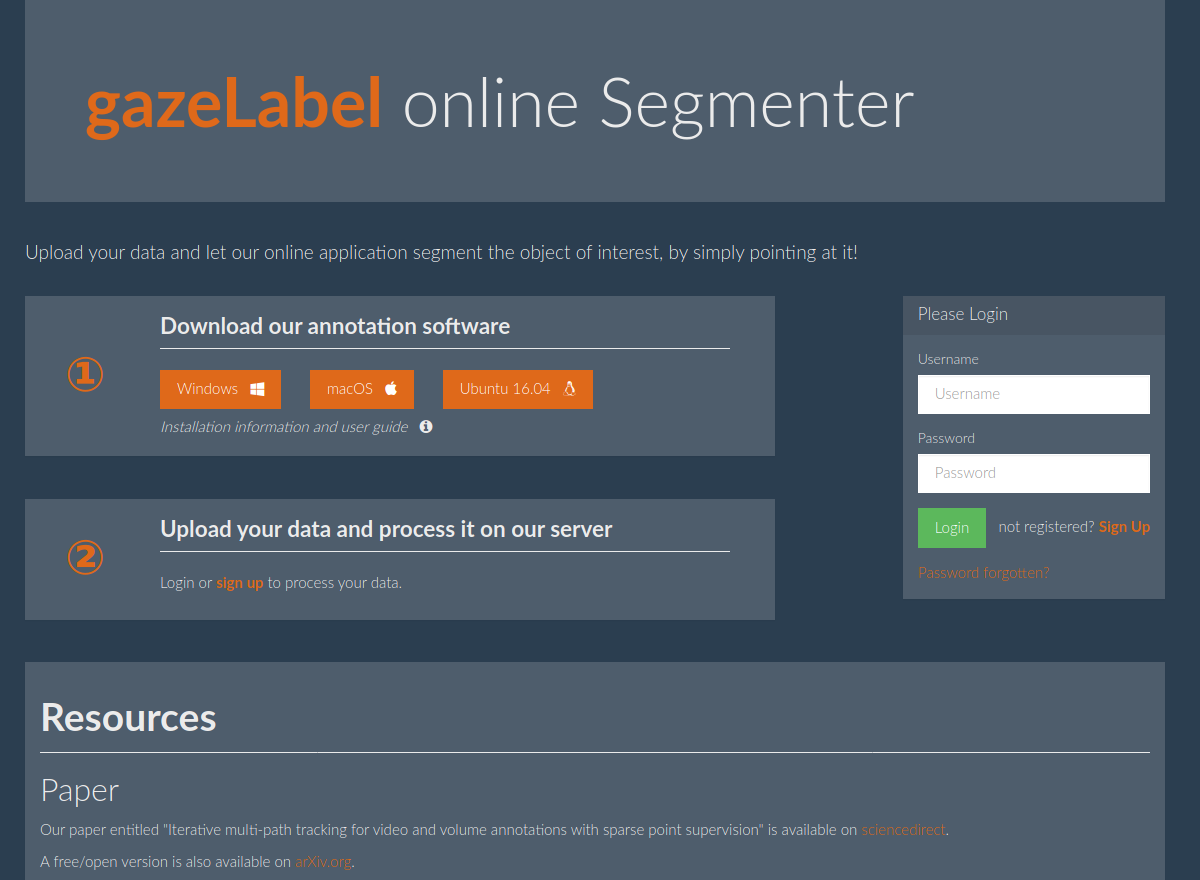
\includegraphics[width=0.99\textwidth]{gazelabel.png}
  \caption{Screenshot of our web platform. Home page.}
  \label{fig:homepage}
\end{figure}

The frontend, which generates the web pages uses the \href{https://webpack.js.org}{Webpack} bundler.
The backend is based on the \href{https://www.djangoproject.com/}{Django} framework, which handles different applications, namely the forms (login, data upload), the task queue, and the database.
Also, the backend is able to trigger a segmentation script on a remote instance and receive the results.

\begin{figure}[!htpb]
  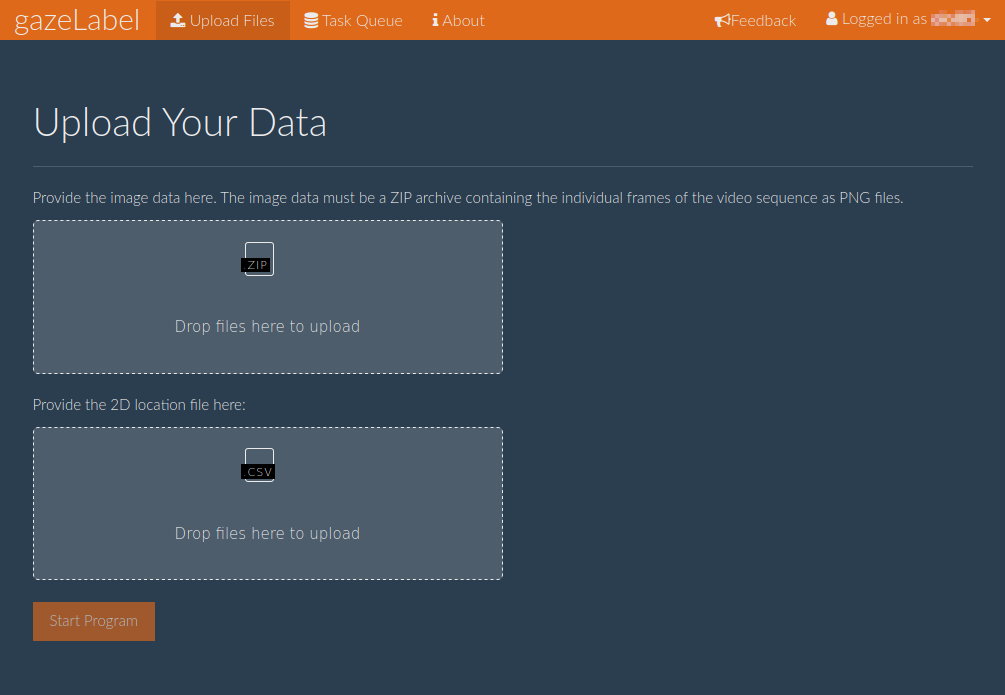
\includegraphics[width=0.99\textwidth]{gazelabel_upload.png}
  \caption{Screenshot of our web platform, where the user can upload a sequence and its corresponding annotations. The task queue panel shows the state of the submitted tasks.}
  \label{fig:upload}
\end{figure}

%%% Local Variables:
%%% mode: latex
%%% TeX-master: "../../main"
%%% End:
